\documentclass[12pt]{article}
\usepackage{titlesec}
\usepackage{setspace}
\usepackage{graphicx}    % needed for including graphics e.g. EPS, PS
\usepackage[left=1.5in,top=1in,right=1in,bottom=1in]{geometry}
\textwidth 6in
\textheight 9in
%\pagestyle{empty}       % Uncomment if don't want page numbers
\parskip 7.2pt           % sets spacing between paragraphs
%\renewcommand{\baselinestretch}{1.5} % Uncomment for 1.5 spacing between lines
\parindent 0pt		 % sets leading space for paragraphs
\titleformat{\section}{\bfseries}{\thesection}{12pt}{}
\newcommand{\sectionbreak}{\clearpage}
\begin{document}         
% Start your text

\section{Abstract}
\label{Abstract}
\doublespacing

In this thesis, I blabber about stuff I think is interesting and apply mountains of computer power that would have been the envy of world militaries 20 years ago to build a go engine with less skill than a drunk macaque.

\title{Application of Stacked De-Noising Auto-Encoders to Planning}
\section{Motivation}

I was inspired by several researchers with ideas about the brain. Jeff Hawkins, who argues that the neocortex is uniform in structure yet represents a hierarchy of abstraction, and Daniel Wolpert, who stresses that the evolutionary purpose of the brain is to produce complex adaptive movements. The synthesis of these ideas leads to the hypothesis that the cortex has a unified process of perception and control where models are biased towards desirable situations and towards information relevant to action. This is somewhat consistent with Perceptual Control Theory as put forward by Bill Powers, which hypothesizes that perceptions are controlled rather than actions, and that action is the result of negative feedback systems bringing the world into agreement with perception. Observations in psychology such as the self-serving and confirmation cognitive biases support this view. We recall the world being closer to our own model than it really is, and our model is biased towards scenarios that would benefit us. This may an artifact of a beneficial adaptation: the brain's unification of perception and control in the neocortex. Under this hypothesis, we do not have a model of the world, and a set of goals from which we derive plans, as classical AI has sought to build. We have a single biased model which simultaneously represents both imperfectly. This model is hierarchically organized into levels of abstraction, and each level learns by roughly the same process. It is possible that the most abstract levels are more representative of goals than of the world, but each level is still permeated with bias to some extent. I elaborate on this model in Section~\ref{fart}. These ideas about how the brain might learn and perform perception and control seemed idealistic until Geoffrey Hinton's deep belief networks started showing successes in the field of machine vision. These unsupervised learning algorithms can build up levels of abstraction, and given enough computer power, can discover hierarchical latent structure in data. They seem like the perfect candidates for the scaffolding of a new model based on the ideas of all these scientists. 
 
	\subsection{Jeff Hawkins' ideas about the neocortex}
	
Jeff Hawkins, notable founder of Palm Computing, Handspring, and Numenta, has written extensively about his Memory-Prediction model of the mammalian neocortex. It can be summarized as follows: The Central Nervous System (CNS) consists of the cortex and lower brain structures. The lower brain structures produce movements by reflex with added noise. The cortex collects the signals sent out of the CNS and the sensory signals coming in from senses. It consists of sheet of functionally similar tissue, loosely subdivided into regions, each of which learns a predictive model of it's receptive field. Receptive fields can consist of sensory inflow, motor outflow, and predictions from other regions. Each region will actively predict the state of it's receptive field, passing those predictions down to those other regions in it's receptive field, and up, to any regions who's receptive field they are in. The global structure of the connections is a hierarchy, with large subtrees for each sense, and with an upper level where sensory integration occurs, containing mostly regions that predict abstract invariant representations.

	\subsection{Daniel Wolpert's ideas about the motor-control purpose of the brain}
	
Daniel Wolpert studies sensorimotor integration and uses engineering methods to model how the CNS controls movement. He stresses that motor control is the adaptive purpose of the brain, because all of the brain's effects on the world are mediated through contractions of the muscles. Only organisms that move have brains, so it stands to reason that motion is closely connected to the brain's adaptive purpose. He and his team developed a model based on Kalman filters where the CNS makes simultaneous predictions of future sensory inputs and future motor outputs with the same process.
	
	\subsection{Geoffrey Hinton's Recent successes with Deep Belief Networks}
	
Geoffrey Hinton, while he was at the University of Toronto, and recently, at Google, has been a pioneer in the field of Deep Belief Networks. These networks feature a layered network topology and methods for training them, that out-perform flat networks with an equal number of trainable parameters. Many types of learning modules can be stacked into a deep network. Hinton and his team have focused primarily on restricted Boltzmann machines (RBMs) and Stacked de-noising auto-encoders (SdAs)

	\subsection{Bill Powers and Perceptual Control Theory}

Perceptual Control Theory is a formalized model of how an organism might control it's behavior. Specifically, It does not control it's behavior, it controls it's perceptions

	\subsection{Computational growth and the promise of scalable flexible hierarchies}
	
It remains to be seen whether these deep learning algorithms can be applied successfully to motor control, high-level planning, and the many other functions we know the neocortex is involved in. Moving forward in the search for artificial general intelligence it is important that we test new algorithms on the same variety of tasks as we know the brain to be capable of solving, and that we test them at the same scale in realistic environments, to the extent that sufficient computer power is affordable. A scalable algorithm which has mediocre performance on a variety of tasks with today's computing power is more promising as a model of the brain than an algorithm that excels at only one task.
	
	\subsection{The unification of perception and planning within the framework of deep nets.}
	\label{fart}

Classical AI has a neutral model of the world and a set of goals. Plans are derived from the combination of these two elements. I'm proposing that a successful biologically inspired learning algorithm could have only one model, biased towards desirable situations, which would represent the world, and the goals, simultaneously, and imperfectly. The benefit of this is it's simplicity, scalability, and self-similarity. In this model, a deep net would would be pre-trained on observations of the world and of one's own actions which are initially random. The system would then transition to a period of fine-tuning where desirable outcomes are enforced from the top down. Sensory information propagates up the network, and desirability-biased expectations propagate down the network. Each layer performs the same task, it modifies it's weights by a gradient based on a combination of data from below, and expectations from above. At the bottom, the data is ground truth, and any data about one's own actions becomes ground truth by taking those actions. At the top, the expectations are set explicitly by the programmer. 

If a modern deep belief network can be made to perform planning tasks, then I believe it lends strength to the biological plausibility of that algorithm. I am operating on the assumption for this project, that perception and planning are both part of the same process, so the most abstract representations are joint models of sensory experience and action. The model of sensory data is influenced by three main factors. The accuracy, the sparsity, and the desirability, or pleasurableness to the creature. At all levels, the representations which jointly satisfy these three metrics come to dominate. In the case of a game this last factor would be the points or wins/losses experienced by the player. The player perceives the state of the game and the state of it's own recent actions, and expects a likely, sparse, and desirable scenario next, and then is made to take any actions it expected of itself which are legal in the rules of the game. 
		
\section{Background}
	\subsection{Deep belief nets}
	
The reason deep belief networks offer some benefit over a completely flat network with the same number of trainable parameters is that they can generalize at different levels and thus share more information. For example, a flat network which has learned a mapping between pictures of cars and labels cannot re-use any of those weights to learn a mapping between pictures of animals and labels. However, a deep network with an intermediate layer sensitive to edges could be shared between them and both classifiers could then be expressed with a far smaller number of weights, as all natural images can be more compactly represented as collections of edges. 

	\subsection{Auto-encoders}
	
Autoencoders, or autoassociators as they are sometimes called, are a variant of the simple three-layer artificial neural network where the output is expected to equal the input and the hidden layer is smaller or sparser than than the input layer. % Split this up. What is a three layer artificial NN? Does the last clause refer to Autoencoders specifically?
An autoencoder takes an input $\mathbf x\in[0,1]^d$ and first maps it (with an encoder) % I'd take out that parenthetical or explain some of this language. What does hidden mean here?
to a hidden representation $\mathbf y\in[0,1]^{d'}$ through a deterministic mapping, e.g.:

\[
\mathbf y = s(\mathbf W\mathbf x + \mathbf b)
\]
Where $s$ is a non-linearity such as the sigmoid. % the sigmoid function?
The latent representation $\mathbf y$, or code is then mapped back (with a decoder) into a reconstruction $\mathbf z$ of same shape as $\mathbf x$  through a similar transformation, e.g.:
\[
\mathbf z = s(\mathbf W'\mathbf y + \mathbf b')
\]
$\mathbf z$ should be seen as a prediction, or {\it reconstruction}, of  $\mathbf x$ given the code  $\mathbf y$. The parameters of this model ($\mathbf W$, $\mathbf W'$, $\mathbf b$, and $\mathbf b'$) are optimized such that the average reconstruction error is minimized\cite{Bengio09}.

The aim of the autoencoder to learn the code $\mathbf y$ a distributed representation that captures the coordinates along the main factors of variation in the data (similarly to how principal component analysis (PCA) captures the main factors of variation in the data). Because $\mathbf y$ is viewed as a lossy compression of $\mathbf x$, it cannot be a good compression (with small loss) for all $\mathbf x$, so learning drives it to be one that is a good compression in particular for training examples, and hopefully for others as well, but not for arbitrary inputs. That is the sense in which an auto-encoder generalizes: it gives low reconstruction error to test examples from the same distribution as the training examples, but generally high reconstruction error to uniformly chosen configurations of the input vector.

If there is one linear hidden layer (the code) and the mean squared error criterion is used to train the network, then the  hidden units learn to project the input in the span of the first  principal components of the data. If the hidden layer is non-linear, the auto-encoder behaves differently from PCA, with the ability to capture multi-modal aspects of the input distribution. The departure from PCA becomes even more important when we consider stacking multiple encoders (and their corresponding decoders) when building a deep auto-encoder [Hinton06].

The auto-encoder alone is not sufficient to be the basis of a deep architecture because it has a tendency towards over-fitting. The denoising autoencoder (dA) is an extension of a classical autoencoder introduced specifically as a building block for deep networks\cite{Vincint08}.  It attempts to re-construct a corrupted version of the input, but the error in $\mathbf z$ is still compared against the un-corrupted input. The stochastic corruption process consists in randomly setting some of the inputs (as many as half of them) to zero. Hence the denoising auto-encoder is trying to predict the corrupted (i.e. missing) values from the uncorrupted (i.e., non-missing) values, for randomly selected subsets of missing patterns. This modification allows the dA to generalize well and produces compounding benefits when the dA's are stacked into a deep network\cite{Hinton06}. Hinton (google tech talk 3) suggests that the stochastic timing of the action potentials observed in biological neurons is a similar feature evolved to moderate the potential for over-fitting, and allow neurons or neuron groups to generalize well over the range of activation patterns of their receptive fields.

	\subsection{Stacked De-noising Auto-encoders}
	
Stacked denoising autoencoders, canonically abbreviated SdA, are not just neural networks with additional hidden layers, but a structure with individual levels of simple three-layer denoising autoencoders. First, a single denoising autoencoder is trained on the data. It's hidden layer converges on a sparse distributed representation of the training set. This essentially replaces the step where a researcher would have to design a collection of good features. Then, a second denoising autoencoder is trained to reconstruct corrupted versions of the activation of the hidden layer of the first dA for the collection of training examples. (the first level does not learn during this time). After a sufficient number of levels have been added, if the network is to be used for classification, the encoders and decoders from each level are assembled into one long network and fine-tuned using back-propagation.

	\subsection{The game of Go}
	
Go is a two-player strategy game, like chess but thousands of years older, simpler rules, and more difficult to master. Players alternate by placing white and black stones on the intersections of a 19 by 19 board. Stones cannot be moved after being placed, but they can be captured and removed if they are surrounded. The goal is to surround more territory than the opponent and capture his stones. The score at the end of the game is the territory surrounded plus captures. Go is known for it's simple rules, yet complex play. It takes only minutes to learn how to play, but years to master. On top of that, it has an astronomically large game-tree complexity. Typically there are between 50 and 300 legal moves available at any state in a game of go, and games typically last about 250 moves but are potentially much longer. Its game-tree complexity ranges from about $\mathbf 10^{600}$ to $\mathbf 10^{800}$. This is hundreds of orders of magnitude larger than chess, and modern supercomputers (approx. 1 PFLOP) can only exhaustively look ahead around 5 moves. It draws much attention from computer programmers because of it's numerical difficulty, and alluring simplicity. The definitions of terms and rules are as follows:

A group is a set of orthogonally connected stones.
Liberties are the unoccupied spaces bordering a group.
Groups with no remaining liberties is considered dead.
When you play a stone, any of your opponents groups that have zero liberties are captured and removed.
One cannot play a dead stone or kill one's own group.
One cannot return the board to a prior state.
Three consecutive passes ends the game.
The score is the sum of surrounded territory plus captures plus the komi for white (an empirically determined handicap of about 6.5 points to offset black's advantage from going first)

There is often another rule listed: a group with two eyes (surrounded empty space) is unambiguously alive. However, since this is derivable from the other rules, it's not necessarily a rule. Also, players often agree that a group without two eyes is alive, because it is extensive or well defended. The invader basically admits that he/she could not capture it and will not try. But if an opponent is trying to surround your group and capture it, you better form two eyes quick. It then becomes safe because in order to theoretically capture it, your opponent would have to totally fill in both eyes, and they would have to fill in one of them first, meaning that they would have to play a dead stone at some point, which is illegal. After you form two eyes, a rational opponent will immediately give up trying to capture your group. This leads to the strategy of fooling beginners into wasting a bunch of moves surrounding your group, only for you to form two eyes at the last second.

\section{Experimental Design}
	\subsection{Choice of Deep Belief Network}
	
Why I'm using SdAs
		
	\subsection{Choice of planning task: the game of Go}

Why was Go chosen? it is a difficult game for computers, with a huge branching factor. This ensures that brute force is infeasible and rules out the possibility of it being used in-whole or in-part. Go requires planning at different scales of time and space. Sometimes sacrifice is strategic. Neither a purely greedy or purely sustainable outlook is as good as a balance between the two.
	
	\subsection{Acquiring and preparing the data-set}
	
To construct the dataset, I first collected tens of thousands of recorded go games as SGF files from the IGS server and other sources such as professional tournaments. I then filtered out about 20 percent of those games because they were in incomplete or were played by nonstandard rules. Then each move in each games was recorded as a training example. Training examples were vectors of 363 numbers between 0 and 1. The first 361 numbers were the board positions of the 19x19 board. an empty position was represented with 0.5, while a white or black stone was represented with 0.75 or 0.25 respectively. The last moves of white and black were represented with 0 and 1 respectively. I chose not to represent the last moves as normalized coordinates because that would make them sensitive and would create a very non-smooth space for the most important parameters in the model. Finally, the last two numbers are the normalized clamped game move number and the final score for black. In each game, the moves of both players are used to create training examples but white's moves are inverted because all moves are stored from black's perspective and when the engine plays go, if it plays as white, it inverts the state to present it to the SdA.

Overall, 1.9 million training examples were created. This dataset was then divided randomly into training, test, and validation sets. 4/5ths of the initial set was used as training data, 4/5ths of what remained was test data, and the remaining part was the validation set. The dataset could not fit in main memory so it was randomized using parallel external merge sort of murmur3 hashes of the training example indices plus a constant seed offset. The randomized data were divided into 1 Gb chunks and stored on an SSD for fast loading into the GPU.
	
	\subsection{Greedy layer-wise pre-training}

The SdA was pre-trained on a dataset of 1,922,933 go positions from the color perspective of the winner. Only the moves in which the winner just places a stone were used. This is the sense in which the SdA preferentially remembers desirable situations, as opposed to remembering all situations in an unbiased model of reality and then deriving actions from the model and a goal. One attempt was made to modify the learning rate with respect to the game's final score on a point by point basis, but it was core-limited as it required communication between the CPU and GPU on every data point, and at the speed of one core, the training process would not have finished for several months. In order to fully take advantage of the GPU and finish in a reasonable amount of time, additional optimizations would have to be designed specifically for this application.

The network topology used was [363, 250, 150, 50, 10]. Each denoising autoencoder in the SdA was trained for 100 iterations of the entire dataset. The entire SdA has about $\mathbf 2^{18}$ trainable parameters.
	
	\subsection{Goal-oriented fine-tuning}


	
	\subsection{Implementation of go engine}

A standard go engine is a computer program which can speak GTP (Go Text Protocol) and decide on moves from game states. Through a bit of wrapper code, it connects to a go server like KGS or a local game arbitration software where it plays games against humans or other go engines. I used an excellent local go engine manager and go library called Gomill by Matthew Woodcraft. %reference

The go engines takes a game state from the current game, and creates a vector of floats from it in the same way that the dataset training examples were created. An empty space is represented as a 0.5, a stone of one's own color represented with a 0.25, a stone of the other player represented with a 0.75. Ones own last move (in the training examples) is represented with 0.0 and the opponents last move with a 1.0. There are two other numbers added. the move number / 200 and the final score from one's own color's perspective. The SdA's encoder weights are used to propagate the activations up to the highest hidden layer, and then the decoder weights are used to propagate those activations back down to the board's state. It is hoped that the resulting prediction will resemble the board state the network was primed with, plus the information about the "last move" made by the current player, which was always present in the training data. At this point, the legal board position with the minimum predicted value is taken to be the choice move and the play is made. The Gomill library handles the GTP protocol from there on.
	
	\subsection{Testing of go engine against various other oponents}
	

	
\section{Results}
	\subsection{Analysis and visualization of hidden units}
		Did the system have abstract representations of perceptions
		Did the system have abstract representations of actions.
		
By observing played games, creating visualizations of the hidden nodes in the network, we can try to get an idea of how the SdA is encoding the data, and whether it has converged on abstract representations of typical Go patterns, and whether it can be said to have "plans".
		
\begin{figure}[htb]
\begin{center}
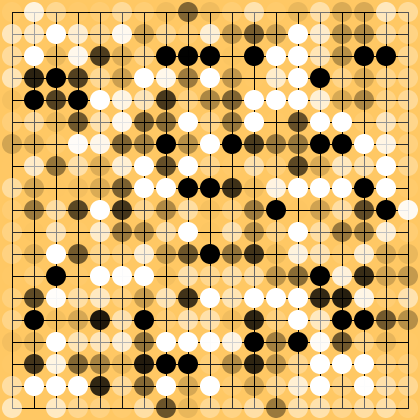
\includegraphics[height=3.0in,width=3.0in]{screen-0204}
\caption{A representation of the go position that would maximally activate one of the hidden units from the highest level in the SdA. Stones are either colored white or black based on the direction of the prediction, and the opacity is the confidence that a stone would be in that position rather than being empty.}
\end{center}
\end{figure}
		
	\subsection{Performance of Go engine}
	
Testing the go engine against GNU Go level 1, I found that after 10,000 games, it lost every single game, even with a 10 point handicap. It is completely incapable of playing go. After playing a game with it manually, I found that while it displayed good placement and coverage at beginning of the game, it the did not try to save groups from atari (the condition of being only one turn from death) which makes it very easy to beat by hundreds of capture points. It also does not refrain from placing stones within it's own territory, needlessly reducing it's own score, and will sometimes fill a large surrounded area with stones of it's own color until only one liberty remained, leading to the capture of that group, and massive losses. It is designed to learn when to pass, but it did not appear to ever pass strategically, it would only pass when there were no more legal moves. 

I decided to use go as a planning task because it has simple rules, a large dataset was readily available, and typical strategies can be decomposed into abstract levels. However, playing adequate go is a very difficult problem to solve programmatically, and GNU go is a very mature and widely reviewed go engine. It is possible that my representation of the game states or my method of training does not present this problem to the autoencoder in a readily digestible way. Or that the go engine does not adequately exploit the SdAs learned representation. It could be that the SdA is too small, or the dataset is too sparse. Whatever the case it is very difficult to diagnose, and much more experimentation would be needed to produce an adequate go engine with this method. This, I believe is weak evidence for the null hypothesis, that SdAs cannot engage in planning in this way. Presumable, some other configuration would be successful, but that is the problem with all AI research. It is difficult to know which methods to pursue, because you can look at any method and say, "If I could only work on that another month I could get some great results" The road ahead is always clouded by fog, and only by sending feelers out in every direction can we discover new solutions.
	
\section{Discussion and Potential Improvements}
	\subsection{Other choices of problems}
	
A simpler problem directed at the issue of learning a sensorimotor task would be more appropriate for determining whether a deep network could plan in this way. For example, moving a limb through a two dimensional space, or solving the Towers of London task.
	
	\subsection{Why it didn't work}
	
Most likely, the search space was too vast and spiky. SdAs are not magic invariance-finding systems. While they are definitely more impressive than past algorithms on perception tasks, they apparently can not be simply pointed at any data and be expected to learn a sparse representation. A sufficiently large amount of data is needed, and sufficient computing resources must be supplied. The data must be somewhat smooth and represented in an learnable way. On top of that, an appropriate network topology must be used. All these factors make it difficult to know what wen't wrong, but still, SdAs are a step in the right direction. Maybe one day we will have learning algorithms that can simply be pointed at any data and will discover invariant representations, after all that's what the brain does.
	
	\subsection{Scale of the problem and difficulty of visualization}
	

	
	\subsection{Other representations of the dataset and actions}
	
	
	
	\subsection{Conclusion}



\begin{thebibliography}{99}
\singlespacing

\bibitem{Somebody09} asdasdasd

\end{thebibliography}
\end{document}